\section{Mutability and Types}


\subsection{Mutability as a Permission}

Logically, it is possible to represent mutability as a {\em permission tag} that may be present as a type member. See listing~\ref{lst:mutability-as-tag} for a hypothetical example. On the left, there is a type containing a single declared member {\cd foo}. On the right, there is a type containing both {\cd foo} and the permission tag {\cd <mutable>}.

The presence of a permission tag on a type allows certain operations to be performed on objects of that type, and conversely, the absence of a permission tag prevents certain operations from being performed. Specifically, the absence of the {\cd <mutable>} permission on type {\cd T1} prevents assignment to any field of an object typed {\cd T1}, and it also prevents any read of such a field from returning a reference that contains the {\cd <mutable>} permission.

\begin{lstlisting}[float=htbp, caption={Mutability as a Permission Tag}, label={lst:mutability-as-tag}]
Type Without Mutability Permission     Type With Mutability Permission
----------------------------------     -------------------------------
type T1 = {                            type T2 = {
  var foo: U                             var foo: U
}                                        permission <mutable>
                                       }
\end{lstlisting}

The right type~{\cd T2} is a subtype of the left type~{\cd T1}, at least under a structural typing regime. (Under a nominal regime, we may not be able to determine this particular subtype relationship because {\cd T1} and {\cd T2} are not related by inheritance. However, the approximations made by a nominal regime are not relevant to the present discussion.)

%The presence of the {\cd <mutable>} permission on type {\cd T2} increases the size of the set of possible operations that are safe to perform relative to {\cd T1}, and since an increase in the number of safe operations generally indicates a more specific type, we can reasonably say that {\cd T2} is a subtype of {\cd T1}.

\subsection{Mutability as a Trait}

Rather than implementing the mutability permission literally as a type member, in the present work I explore the possibility of implementing the mutability permission as a trait/mixin.
The {\cd MutableAny} trait represents the presence of the mutability permission, and mutability can be added to any type by means of {\em type intersection}. Type intersection in Dotty can be done with either the {\cd with} keyword or the amperstand type-intersection operator {\cd \&}.
For example, listing~\ref{lst:intersection-mutableany} shows two ways of defining a type~{\cd U} as a mutable version of type~{\cd T}.
Type~{\cd U} logically contains all of the same members as type~{\cd T}, as well as the mutability permission.

\begin{lstlisting}[float=htbp, caption={Intersection with MutableAny}, label={lst:intersection-mutableany}]
type U = T with MutableAny
type U = T & MutableAny
\end{lstlisting}

Type intersection is the basic mechanism for adding mutability permissions to a type.

\subsection{Revoking Mutability Permissions}

It is sometimes necessary to build types where mutability permissions have been revoked.
The revocation of mutability is done by means of a {\em type union}, which is expressed in Dotty by the vertical-bar type-union operator~{\cd |}, as in listing~\ref{lst:union-readonlynothing}.

\begin{lstlisting}[float=htbp, caption={Union with ReadonlyNothing}, label={lst:union-readonlynothing}]
type U = T | ReadonlyNothing
\end{lstlisting}

The {\cd ReadonlyNothing} trait requires some explanation. {\cd ReadonlyNothing} is assumed to contain all possible members, except for the mutability permission. The type union operation preserves only those members that are common to both operands, so type~{\cd U} in listing~\ref{lst:union-readonlynothing} contains exactly the set of members as type~{\cd T}, except for the mutability permission.

\subsection{Default Mutabilities} \label{sec:default-mutabilities}

Most types are considered mutable by default.

The only types that are not mutable by default are {\cd Any} and {\cd ReadonlyNothing}.
The non-mutability of {\cd ReadonlyNothing} is self-explanatory, but the non-mutability of {\cd Any} requires some explanation.

In a cursory examination of practical code, I have seen three dominant uses of {\cd Any}: first, as the upper bound of an abstract type parameter; second, as the type of a method parameter that may be dynamically downcast within the method; and third, as the element type of a container. Listing~\ref{lst:dominant-uses-of-any} shows examples of these uses.

\begin{lstlisting}[float=htbp, caption={Dominant Uses of the Any Type}, label={lst:dominant-uses-of-any}]
class List[E] { ... }                         // Case 1

def m(x: Any) = x match { case x: T => ... }  // Case 2

val map: Map[String, Any]                     // Case 3
\end{lstlisting}

In case~1, the abstract type parameter~{\cd E} is not assigned an explicit upper bound, so a default upper bound of {\cd Any} is assumed. In case~2, the method parameter~{\cd x} is dynamically cast to a subtype before any possibly-mutating methods are called. In case~3, {\cd Any} is used as an opaque type, allowing storage and retrieval of arbitrary objects. In none of these cases is a mutating method called directly on an object with type {\cd Any}.

The only potentially problematic case is case~2, where {\cd Any} is downcast to another type.
If {\cd Any} is assumed to be {\em readonly}, then preservation of static reference-immutability guarantees requires that all downcasts of~{\cd x} are also readonly.
Otherwise, a downcast may unintentionally permit a mutation that should have been prohibited.

An alternative is to consider {\cd Any} to be a mutable type, and introduce a different (readonly) top type. Unfortunately, there is a pervasive assumption in the Dotty compiler that {\cd Any} is the top type. Attempting to change this assumption to support case~2 code examples seemed like it would create more problems than it would solve.

Ideally, the type of parameter~{\cd x} in case~2 would be {\cd MutableAny} rather than {\cd Any}. In practice, generating errors for code like case~2 would force programmers to perform the replacement of {\cd Any} by {\cd MutableAny} manually, unless some kind of automatic replacement is done.

It is possible to automatically substitute explicit uses of {\cd Any} with {\cd MutableAny} at compile time, which will perhaps go most of the way toward allowing legacy code to compile as-is. Such a substitution would affect the uses of {\cd Any} in cases~2 and~3, but not the default upper bound of type parameter~{\cd E} in case~1.

\subsection{Type Lattice}

The default Dotty type lattice is as shown in figure~\ref{fig:default-type-lattice}. {\cd Any} is a supertype of all other types, and {\cd Nothing} is a subtype of all other types.

\begin{figure}[htbp]
\center
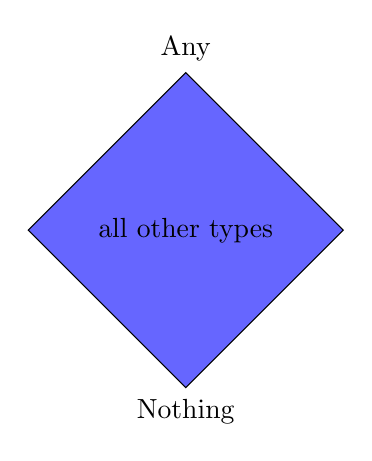
\begin{tikzpicture}
	\filldraw[fill=blue!60, draw=black] (0, 2) -- (2, 0) -- (0, -2) -- (-2, 0) -- cycle;
	\draw (0, 2.3) node{\cd Any};
	\draw (0, 0) node{\cd all other types};
	\draw (0, -2.3) node{\cd Nothing};
\end{tikzpicture}
\caption{Default Type Lattice}
\label{fig:default-type-lattice}
\end{figure}

\begin{figure}[htbp]
\center
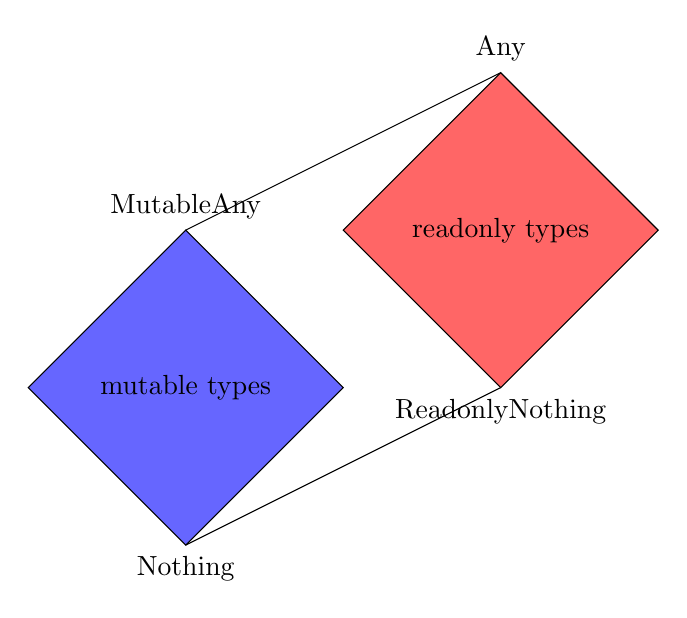
\begin{tikzpicture}
	\filldraw[fill=red!60, draw=black] (0, 2) -- (2, 0) -- (0, -2) -- (-2, 0) -- cycle;
	\draw (0, 2.3) node{\cd Any};
	\draw (0, 0) node{\cd readonly types};
	\draw (0, -2.3) node{\cd ReadonlyNothing};

	\filldraw[fill=blue!60, draw=black] (-4, 0) -- (-2, -2) -- (-4, -4) -- (-6, -2) -- cycle;
	\draw (-4, 0.3) node{\cd MutableAny};
	\draw (-4, -2) node{\cd mutable types};
	\draw (-4, -4.3) node{\cd Nothing};

	\draw[black] (-4, 0) -- (0, 2);
	\draw[black] (-4, -4) -- (0, -2);
\end{tikzpicture}
\caption{Type Lattice with Mutability}
\label{fig:type-lattice-with-mutability}
\end{figure}

When mutability is added, the lattice is extended to include two versions of each type: one with the mutability permission, and one without. For every mutable type, there is a readonly supertype that is identical except for the absence of the mutability permission. Figure~\ref{fig:type-lattice-with-mutability} shows the extended lattice graphically.

Legacy code assumes the type lattice shown in figure~\ref{fig:default-type-lattice}. The relationships in the lower diamond of figure~\ref{fig:type-lattice-with-mutability} (the ``mutable types'') are identical to the relationships in the ``all other types'' diamond of figure~\ref{fig:default-type-lattice}, allowing legacy code to compile cleanly (modulo some special handling of the {\cd Any} type, as discussed in section~\ref{sec:default-mutabilities}).

The distinction between {\cd Nothing} and {\cd ReadonlyNothing} is important. Most types represent the {\em presence} of members or permissions, but {\cd ReadonlyNothing} represents the {\em absence} of a permission. The idea of using {\cd Nothing}-like types to express the absence of members may be worth exploring further in future work. In the present work, I restrict investigation of {\cd Nothing}-like types to the use of {\cd ReadonlyNothing} for permission removal.

%Although it is not possible to construct an object of either type, 

%It is not possible to construct an object of type {\cd Nothing}, nor is it possible to construct an object of type {\cd ReadonlyNothing}. 

\subsection{Viewpoint Adaptation of Fields}

Type unions and intersectionsare used to perform viewpoint adaptation of field reads.
Given a reference~{\cd t} of type~{\cd T}, and a field~{\cd u} of type~{\cd U}, the type of \mbox{\cd t.u} is:
\begin{figure}[h]
\center
{\cd T \& ReadonlyNothing | U}
\caption{Viewpoint Adaptation (Field Type {\cd U} with Prefix {\cd T})}
\label{fig:viewpoint-adapted-type}
\end{figure}

The expression \mbox{\cd T \& ReadonlyNothing} produces the greatest lower bound of~{\cd T} and {\cd ReadonlyNothing}. Referring the the type lattice in figure~\ref{fig:type-lattice-with-mutability}, the lower bound of~{\cd T} and {\cd ReadonlyNothing} is minimally {\cd Nothing} and maximally {\cd ReadonlyNothing}. The minimal result {\cd Nothing} occurs where~{\cd T} is mutable, and the maximal result {\cd ReadonlyNothing} occurs where~{\cd T} is readonly. The expression {\cd T \& ReadonlyNothing} is therefore a way to ``extract'' the mutability permission from~{\cd T} while ignoring all other members of~{\cd T}.

The subsequent union with type~{\cd U} finds the least upper bound of \mbox{\cd T \& ReadonlyNothing} and~{\cd U}. The result is minimally just~{\cd U}, and maximally \mbox{\cd ReadonlyNothing | U}, which is equivalent to~{\cd U} without any mutability permission.

The viewpoint adaptation formula in figure~\ref{fig:viewpoint-adapted-type} protects the transitive reference-immutability guarantee.
The mutability of the viewpoint-adapted type is the least upper bound of the mutabilities of~{\cd T} and~{\cd U}, which means that it cannot be less restrictive with respect to mutability than either~{\cd T} or~{\cd U}.

\subsection{Polymorphic Mutability Types}




\begin{comment}

\subsubsection{Discussion of Alternatives: Dynamic Permissions}

The focus of the present work is on static checking of mutability permissions, but an alternative direction would have been to provide dynamic support for mutability permissions. Although I do not implement or evaluate dynamic mutability permissions in the present work, the idea is perhaps worth a very brief discussion.

\begin{lstlisting}[float=htbp, caption={Permission Tag Example}, label={lst:permission-tag-example}]
type T2 = {
	var foo: T2 = this
	permission <mutable>
}
type T1 = {
	var foo: T2 = this
}
val t = new T2()
t.foo                      // result contains permission <mutable>
t.asInstanceOf[T1]         // result does not contain permission <mutable>
t.asInstanceOf[T1].foo     // result does not contain permission <mutable>
\end{lstlisting}

Normally, the type of an object is fixed at the time it is created. However, where there is viewpoint adaptation, the observed type of an object depends on the path used to reach that object.

Consider listing~\ref{lst:permission-tag-example}. The reference~{\cd t} refers to a new object that has the {\cd <mutable>} permission. However, if {\cd t} is cast to type {\cd T1} (which is reasonable in a structural regime if not necessarily a nominal one), the type of the resulting reference cannot contain the {\cd <mutable>} permission. Furthermore, 


It is possible that the path-dependence of viewpoint adaptation may be related in some way to the path-dependence of DOT. However, I do not elaborate further on this thought in the present work.

% Translation of mutability permissions into traits/mixins.



The fundamental approach I take here is to treat mutability as a {\em permission} represented by a {\em trait} or {\em mixin}. By representing mutability as a trait, mutability can be added to any type by means of type intersection.

Practically, I introduce a the trait {\cd MutableAny} to represent the presence of the mutability permission. Given any arbitrary type {\cd T}, the mutability permission can be added using either the {\cd with} keyword or the amperstand ({\cd \&}) type intersection operator:

\begin{lstlisting}
type U = T with MutableAny
type U = T & MutableAny
\end{lstlisting}

In either case, the resulting type~{\cd U} is understood to contain all declarations in {\cd T}, as well as the mutability permission. It is reasonable to understand the mutability permission as a declaration that may be present in a type (other kinds of declarations allowed in Dotty are fields, methods, and type members). I did not literally implement permissions as a fourth kind of declaration in Dotty. Although the permission-as-declaration concept is an intriguing possibility for future study, it is too complex of a topic to discuss thoroughly in the present work.

In the present work, {\cd MutableAny} is assumed to contain the mutability permission. Other named classes and traits are also assumed to contain the mutability permission, for the purpose of allowing existing code to compile without modification. The only exception is the top type {\cd Any}, which is {\em not} assumed to contain the mutability permission. Before moving on, I discuss the rationale and tradeoffs involved in the choice to treat {\cd Any} as a readonly type.

\subsubsection{The Any Type as a Readonly Type}

In a cursory examination of practical code, I have seen three dominant uses of {\cd Any}: first, as the upper bound of an abstract type; and second, as the type of a function parameter that may be dynamically cast to a subtype; and third, as the element type of a container. The following are examples of these uses:

\begin{lstlisting}
class List[E] { ... }                         // Case 1

def m(x: Any) = x match { case x: T => ... }  // Case 2

val map: Map[String, Any]                     // Case 3
\end{lstlisting}

In case~1, the type parameter~{\cd E} is not assigned an explicit upper bound, so a default upper bound of {\cd Any} is supplied. In case~2, the method parameter~{\cd x} is dynamically cast to a subtype before any possibly-mutating methods are called. In case~3, {\cd Any} is used as an opaque type, allowing storage of arbitrary objects.

It should be noted here that {\cd Any} is not equivalent to {\cd Object}. In Dotty, {\cd Object} is a reference type, and {\cd Object} is a subclass of {\cd Any}. {\cd Object} is treated as a reference type, and indeed {\cd AnyRef} is an alias of {\cd Object}, allowing a distinction between reference types and primitive types (primitive types extend {\cd AnyVal}). Although the type erasure phase of the compiler converts {\cd Any} and {\cd AnyVal} to {\cd Object} for the purpose of interoperability with Java, the source-level distinction between {\cd Any} and {\cd Object} is convenient for supporting reference immutability. The methods defined by {\cd Any} include {\cd ==}, {\cd toString}, {\cd getClass}, and related methods, which are normally not expected to produce mutations. Methods defined by {\cd Object} include {\cd synchronized}, {\cd finalize}, {\cd notify}, and {\cd wait}, which frequently produce mutations. The reason the distinction between {\cd Any} and {\cd Object} is convenient is that it should be safe to assume that the methods of {\cd Any} never produce observable mutations, so making {\cd Any} readonly by default should not cause any difficulties with preexisting code. None of the 100+ tests in the Dotty compiler test suite (which include the Dotty compiler itself and a substantial portion of the standard library) appear to call any methods at all on references of type {\cd Any}.

Returning to case~2 above, there is the possibility that reference~{\cd x} will be downcast to a mutable type within the match block, and subsequently mutated. Such a mutation may appear to be a problem because the type of~{\cd x} is a readonly type, so normally one would not expect a mutation of~{\cd x} to be possible. However, the only way to match a mutable type case at runtime is if the reference bound to~{\cd x} at runtime does in fact have a mutable type, which would not actually result in a violation of reference immutability.

Unfortunately, it is not possible to rigourously test runtime pattern matching at this time due to the incomplete status of the Dotty compiler. Due to this circumstance, it seems best to me to relegate the implementation and testing of the runtime aspects to future work.

However, it is possible to make some preliminary statements about the implications of allowing readonly references to be downcast at runtime, even though a complete implementation is left for future work. The first implication is that it is impossible to determine the absence of mutations from the method signature alone. That is, a more precise knowledge of runtime types is required to determine whether or not a given method call is in fact free of side effects. Since the primary motivation behind the present work is to aid programmer reasoning, (what guarantees am I actually able to offer the programmer here?)

One of the implications of allowing dynamic matching of mutability permissions is that it is impossible to determine the absence of mutations from the method signature alone. 

Another implication of dynamic mutability matching is that adding mutability-related annotations and type expressions may alter runtime behaviour. A negative consequence of altering runtime behaviour is that type matching operations that worked correctly before adding mutability may fail at runtime if any mistake is made. However, a positive consequence is that the ability to determine mutability at runtime provides the programmer with more flexibility than a purely static mutability system would allow.


---

Judgements on the downcasting of Any:
1. Any must be readonly. There is a pervasive assumption in Dotty that Any is the top type, and introducing a different top type breaks this assumption. There are a large number of uses of {\cd Any} in the standard library. Making readonly types incompatible with {\cd Any} could make substantial portions of the standard library unusable to code that uses readonly references.
2. It is not reasonable to allow dynamic casts of non-mutable references to produce a mutable results. Method signature would no longer statically indicate the absence of side effects.
3. Existing code that downcasts from Any and attempts mutation will fail. The programmer is expected to replace Any with MutableAny in these cases.

Implementation: viewpoint adaptation on asInstanceOf and match cases.

Info:
in typer#typedCase:
	val pat1 = typedPattern(tree.pat, selType)(gadtCtx)
selType is the type of the selector, so what we want is for the types of any variables defined by the pattern to be viewpoint-adapted with selType. We can tell if we're in a pattern by presence of Mode.Pattern in the context.

But how do we know if an identifier is defined in a particular match block?

The Pattern mode.
The Pattern mode is enabled during typing of case patterns.
When a term identifier is encountered in Pattern mode, it is desugared to a Bind:
	{\cd x} becomes {\cd x @ \_}
where {\cd \_} is the Wildcard type. (See method desugar.patternVar)

The typing of Bind trees seems to be the logical place to enforce viewpoint adaptation. A bind associates a name with a type, and the name can be a type name or a term name.
Specifically, it seems that the type of Bind's body is the type we want to viewpoint adapt.

But how to we know what the match selector type is when we get into typedBind?
Answer: the prototype passed to typedBind tells us.
How does this work for more complicated patterns, e.g.: case x@List(y) => ...?
It looks like the prototype of x is the selector type, and the prototype of y is the type argument, but where should y's type be viewpoint adapted?
Look into Applications#typedUnApply, which computes a value ``ownType'', which in the basic case is just the selector type.
It is possible that this problem will resolve itself after receiver-mutability checking is implemented.

\end{comment}
